\documentclass[proposal.tex]{subfiles} 



\begin{document}

%----------------------------------------------------------------------------
\section{Work Completed}\label{sect:workCompleted}
%----------------------------------------------------------------------------
\subsection{What we are doing}
A partial implementation of the logic programming language \progLang{Prolog} is provided by the library \texttt{prolog-0.2.0.1}. One of the objectives is to 
implement monadic unification using the library \cite{unification-fd-lib}. 


\subsection{Unifiable Data Structures}
For a data type to be Unifiable, it must have instances of Functor, Foldable and Traversable. The interaction between different classes is depicted in figure 
\ref{fig:Functor Hierarchy}.

\begin{figure}[h]
\centering
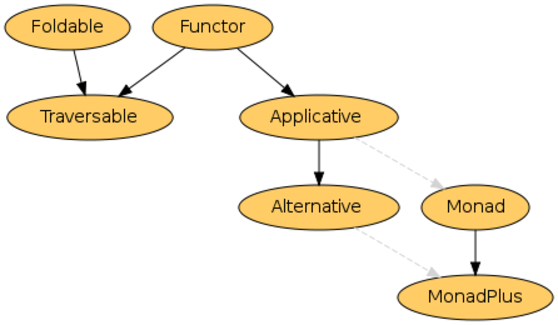
\includegraphics[scale = 0.7]{FunctorHierarchy.png}
\caption{Functor Hierarchy \cite{website:foldablenadtraversable}}
\label{fig:Functor Hierarchy}
\end{figure}  

The Functor class provides the \texttt{fmap} function which applies a particular operation to each element in the given data structure. The Foldable class \textit{folds} the data structure by recursively applying the operation to each element and 

\subsection{Why \texttt{fix} is necessary?}
Since \progLang{Haskell} is a lazy language it can work with infinite data structures. \textit{Type Synonyms} in \progLang{Haskell} cannot be self 
referential.


 

In our case consider the following example,

\begin{minted}{haskell}
-- The Prolog Syntax

type Atom = String

data VariableName = VariableName Int String  deriving (Show,Eq,Ord)

data FlatTerm a = 
		 Struct Atom [a]
	|	Var VariableName
	|	Wildcard
	|	Cut Int deriving (Show,Eq,Ord)
\end{minted} 
 
A \texttt{FlatTerm} can be of infinite depth which due to the reason stated above cannot be accounted for during application function. The resulting type signature would be of the form,

\mint{haskell}|FlatTerm (FlatTerm (FlatTerm (FlatTerm (.....))))|

Enter the \texttt{Fix} same as the function as a data type. The above would be simply reduced to,

\mint{haskell}|Fix FlatTerm|   

resulting in the \progLang{Prolog} Data Type
\mint{haskell}|data Prolog = P (Fix FlatTerm) deriving (Show,Eq,Ord)|

\subsection{Dr. Casperson's Explanation}

A recursive data type in \progLang{Haskell} is where one value of some type contains values of that type, which in turn contain more values of the same type 
and so on. Consider the following example.

\begin{minted}{haskell}
data Tree = Leaf Int | Node Int (Tree) (Tree)
\end{minted} 

A sample \texttt{Tree} would be,

\mint{haskell}|(Node 0 (Leaf 1) (Node 2 (Leaf 3) (Leaf 4)))|

The above structure can be infinitely deep since \progLang{Haskell} is a \textit{lazy} programming language. But working with an infinitely deep / nested 
structure is not possible and will result in a \textit{occurs check} error. This is because writing a type signature for a function to deal with such a
parameter is not possible. One option would be to \textit{flatten} the data type by the introduction of a type variable. Consider the following,

\begin{minted}{haskell}
data FlatTree a = Leaf Int | Node Int a a
\end{minted}  

A sample \texttt{FlatTerm} would be similar to \texttt{Tree}. 

The \texttt{FlatTree} is recursive but does not reference itself. But it too can be infinitely deep and hence writing a function to work on the structure
is not possible.  

The \texttt{fix} function in the \texttt{Control.Monad.Fix} module allows for the definition of recursive functions in \progLang{Haskell}. Consider the 
following scenario,

\begin{minted}{haskell}
fix :: (a -> a) -> a
\end{minted}
The above function results in an infinite application stream,

\begin{minted}{haskell}
f s : f (f (f (... )))
\end{minted} 

A fixed point of a function f is a value a such that f a == a. This is where the name of fix comes from: it finds the least-defined fixed point of a function.








\end{document}